\begin{thm}{101}{\hosi ?}{駿台理系添削指導}
 $\triangle\mr{ABC}$において、$\angle\mr{A}=3\angle\mr{B}$, $\mr{AB}=\sqrt{3}$で、BC, ACの長さはともに整数である。BC, ACの長さを求めよ。
\end{thm}

$\angle\mr{B}=\theta$とおく。$\triangle\mr{ABC}$の内角はすべて正かつ和が$\pi$を超えないことから、$0<\theta<\dfrac{\pi}{4}$である。辺BC上に点Dを、$\angle\mr{BAD}=\theta$となるようにとる。このとき、$\triangle\mr{DAB}$は$\angle\mr{DAB}=\angle\mr{DBA}=\theta$なる二等辺三角形で、$\triangle\mr{CAD}$は$\angle\mr{CAD}=\angle\mr{CDA}=2\theta$なる二等辺三角形である。
\begin{figure}[H]
 \centering
 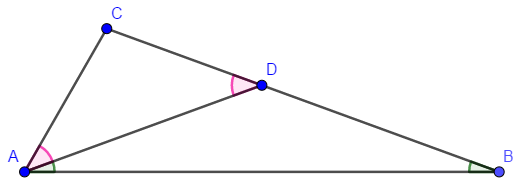
\includegraphics[width=0.7\linewidth]{../problems/Q_101/A_101.png}
\end{figure}
$\mr{AC}=\mr{CD}$が整数、$\mr{BC}$も整数であることから、$\mr{BD}=\mr{AD}$も整数である。$\mr{AD}=\mr{BD}=n$, $\mr{AC}=\mr{DC}=m$とおく。$\sin\angle\mr{ACD}=\sin(\pi-4\theta)=\sin4\theta$となることを踏まえて、正弦定理によって、
\begin{align*}
 \frac{\sqrt{3}}{\sin2\theta}&=\frac{n}{\sin\theta} & &\dou & \cos\theta&=\frac{\sqrt{3}}{2n} \\
 \frac{m}{\sin2\theta}&=\frac{n}{\sin4\theta} & &\dou & \cos2\theta&=\frac{n}{2m}
\end{align*}
倍角公式を用いてさらに整理すると、
\[ \frac{3}{2n^2}-1=\frac{n}{2m} \quad\dou\quad m(3-2n^2)=n^3 \]
を得る。$m, n$はともに正の整数だから、$3-2n^2>0$でなければならない。これを満たす正の整数は$n=1$のみ。このとき$m=1$とわかる。

以上より、$\mr{BC}=m+n=2$, $\mr{AC}=m=1$。